%% what_representation.tex
%% Author: Leighton Pritchard
%% Copyright: James Hutton Institute
%% Summary of Cleveland & McGill, Heer & Bostock studies

% WHAT WORKS BEST? EXPERIMENT
\begin{frame}
  \frametitle{What works best? Experiment
  \footnote{\tiny{\href{https://www.jstor.org/stable/2288400}{Cleveland \& McGill (1984) \textit{J. Am. Stat. Ass.}}}}  
  \footnote{\tiny{\href{http://vis.stanford.edu/files/2010-MTurk-CHI.pdf}{Heer \& Bostock (2010) \textit{CHI 2010}}}}
  }
    \textcolor{hutton_green}{Empirical measurements of interpretation}
    \begin{itemize}  
      \item Subjects shown graphs representing same data
      \item ($\log_2$) Error in subjects' accuracy compared by graph type
    \end{itemize}  
    \begin{alertblock}{Judgement types}
      \begin{itemize}
        \item 1-3: Position on a common scale (bar chart, stacked bar chart)
        \item 4-5: Length encoding (stacked bar chart)
        \item 6: Angle (pie chart)
        \item 7-9: Area (bubble chart, aligned rectangles, treemap) 
      \end{itemize}
    \end{alertblock}
\end{frame}

% WHAT WORKS BEST? RESULT
\begin{frame}
  \frametitle{What works best? Result
  \footnote{\tiny{\href{https://www.jstor.org/stable/2288400}{Cleveland \& McGill (1984) \textit{J. Am. Stat. Ass.}}}}  
  \footnote{\tiny{\href{http://vis.stanford.edu/files/2010-MTurk-CHI.pdf}{Heer \& Bostock (2010) \textit{CHI 2010}}}}
  }
  \begin{columns}[T]
    \begin{column}{5cm}
      \begin{itemize}
        \item \textcolor{hutton_green}{We have inherent biases that can distort information recovered}
        \item \textcolor{hutton_blue}{Position $>$ Angle $\approx$ Length $>$ Area}
        \item Accuracy plateaus as charts increase in size
        \item Gridlines improve accuracy
        \item \textcolor{hutton_purple}{Aspect ratios affect area judgements (squares worst)}
      \end{itemize}
    \end{column}
    \begin{column}{6cm}  
      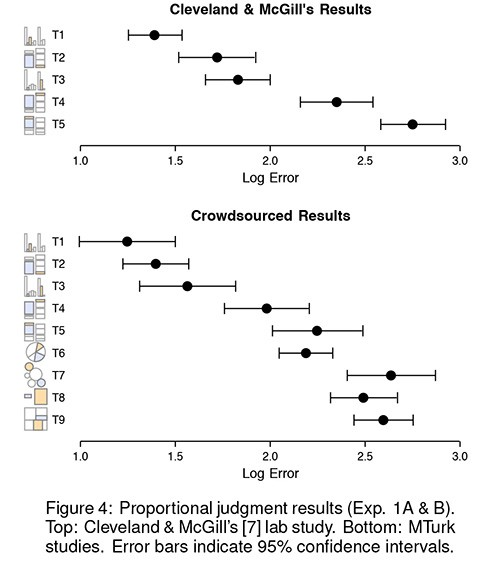
\includegraphics[width=1\textwidth]{images/proportional_results}    
    \end{column}
  \end{columns}      
\end{frame}